	
% This template from http://www.vel.co.nz, originally from http://www.tedpavlic.com

\documentclass{article}
% Change "article" to "report" to get rid of page number on title page
\usepackage{amsmath,amsfonts,amsthm,amssymb, mathrsfs}
\usepackage{bigints}
\usepackage{setspace}
\usepackage{Tabbing}
\usepackage{fancyhdr}
\usepackage{lastpage}
\usepackage{textcomp}
\usepackage{extramarks}
\usepackage{chngpage}
\usepackage{soul,color}
\usepackage{graphicx,float,wrapfig}
\usepackage{cancel}
\usepackage{indentfirst}
\usepackage{mdframed}

% In case you need to adjust margins:
\topmargin=-0.45in      %
\evensidemargin=0in     %
\oddsidemargin=0in      %
\textwidth=6.5in        %
\textheight=9.0in       %
\headsep=0.25in         %

% Homework Specific Information
\newcommand{\hmwkTitle}{WS2}
\newcommand{\hmwkDueDate}{}
\newcommand{\hmwkClass}{Ay\ 190}
\newcommand{\hmwkAuthorName}{Cutter\ Coryell}

% Setup the header and footer
\pagestyle{fancy}                                                       %
\lhead{\hmwkAuthorName}                                                 %
\chead{\hmwkClass\ : \hmwkTitle}  %
\rhead{\hmwkDueDate}                                                     %
\renewcommand\headrulewidth{0.4pt}                                      %
\renewcommand\footrulewidth{0.4pt}                                      %

% This is used to trace down (pin point) problems
% in latexing a document:
%\tracingall

%%%%%%%%%%%%%%%%%%%%%%%%%%%%%%%%%%%%%%%%%%%%%%%%%%%%%%%%%%%%%
% Some tools
\newcommand{\enterProblemHeader}[1]{\nobreak\extramarks{#1}{#1 continued on next page\ldots}\nobreak%
                                    \nobreak\extramarks{#1 (continued)}{#1 continued on next page\ldots}\nobreak}%
\newcommand{\exitProblemHeader}[1]{\nobreak\extramarks{#1 (continued)}{#1 continued on next page\ldots}\nobreak%
                                   \nobreak\extramarks{#1}{}\nobreak}%

\newlength{\labelLength}
\newcommand{\labelAnswer}[2]
  {\settowidth{\labelLength}{#1}%
   \addtolength{\labelLength}{0.25in}%
   \changetext{}{-\labelLength}{}{}{}%
   \noindent\fbox{\begin{minipage}[c]{\columnwidth}#2\end{minipage}}%
   \marginpar{\fbox{#1}}%

   % We put the blank space above in order to make sure this
   % \marginpar gets correctly placed.
   \changetext{}{+\labelLength}{}{}{}}%

\setcounter{secnumdepth}{0}
\newcommand{\homeworkProblemName}{}%
\newcounter{homeworkProblemCounter}%
\newenvironment{homeworkProblem}[1][Problem \arabic{homeworkProblemCounter}]%
  {\stepcounter{homeworkProblemCounter}%
   \renewcommand{\homeworkProblemName}{#1}%
   \section{\homeworkProblemName}%
   \enterProblemHeader{\homeworkProblemName}}%
  {\exitProblemHeader{\homeworkProblemName}}%

\newcommand{\problemAnswer}[1]
  {\noindent\fbox{\begin{minipage}[c]{\columnwidth}#1\end{minipage}}}%

\newcommand{\problemLAnswer}[1]
  {\labelAnswer{\homeworkProblemName}{#1}}

\newcommand{\homeworkSectionName}{}%
\newlength{\homeworkSectionLabelLength}{}%
\newenvironment{homeworkSection}[1]%
  {% We put this space here to make sure we're not connected to the above.
   % Otherwise the changetext can do funny things to the other margin

   \renewcommand{\homeworkSectionName}{#1}%
   \settowidth{\homeworkSectionLabelLength}{\homeworkSectionName}%
   \addtolength{\homeworkSectionLabelLength}{0.25in}%
   \changetext{}{-\homeworkSectionLabelLength}{}{}{}%
   \subsection{\homeworkSectionName}%
   \enterProblemHeader{\homeworkProblemName\ [\homeworkSectionName]}}%
  {\enterProblemHeader{\homeworkProblemName}%

   % We put the blank space above in order to make sure this margin
   % change doesn't happen too soon (otherwise \sectionAnswer's can
   % get ugly about their \marginpar placement.
   \changetext{}{+\homeworkSectionLabelLength}{}{}{}}%

\newcommand{\sectionAnswer}[1]
  {% We put this space here to make sure we're disconnected from the previous
   % passage

   \noindent\fbox{\begin{minipage}[c]{\columnwidth}#1\end{minipage}}%
   \enterProblemHeader{\homeworkProblemName}\exitProblemHeader{\homeworkProblemName}%
   \marginpar{\fbox{\homeworkSectionName}}%

   % We put the blank space above in order to make sure this
   % \marginpar gets correctly placed.
   }%

\newenvironment{myindentpar}[1]%
 {\begin{list}{}%
         {\setlength{\leftmargin}{#1}}%
         \item[]%
 }
 {\end{list}}

%%%%%%%%%%%%%%%%%%%%%%%%%%%%%%%%%%%%%%%%%%%%%%%%%%%%%%%%%%%%%


%%%%%%%%%%%%%%%%%%%%%%%%%%%%%%%%%%%%%%%%%%%%%%%%%%%%%%%%%%%%%
% Make title
\title{\vspace{2in}\textmd{\textbf{\hmwkClass:\ \hmwkTitle}}\\\normalsize\vspace{0.1in}\small{Due\ on\ \hmwkDueDate}\\\vspace{0.1in}\large{\textit{\hmwkClassInstructor\ \hmwkClassTime}}\vspace{3in}}
\date{}
\author{\textbf{\hmwkAuthorName}}
%%%%%%%%%%%%%%%%%%%%%%%%%%%%%%%%%%%%%%%%%%%%%%%%%%%%%%%%%%%%%

%%%% MY COMMANDS %%%%%%%%%%%%%%%%%%%%%

\newcommand{\deri}[2]{\frac{\mathrm{d} #1}{\mathrm{d} #2}}
\newcommand{\pderi}[2]{\frac{\partial #1}{\partial #2}}
\newcommand{\inte}[4]{\int_{#1}^{#2} \! #3 \, \mathrm{d} #4}
\newcommand{\ointe}[4]{\oint_{#1}^{#2} \! #3 \, \mathrm{d} #4}
\newcommand{\del}{\nabla}
\newcommand{\D}{\mathrm{d}}
\newcommand{\ee}[1]{\times 10^{#1}}
\newcommand{\fpe}{\frac{1}{4 \pi \epsilon_0}}
\newcommand{\bra}[1]{\left< #1 \right|}
\newcommand{\ket}[1]{\left| #1 \right>}
\newcommand{\cket}[1]{\left. #1 \right>}


% Distance units
\newcommand{\m}[0]{\text{\ m}}
\newcommand{\cm}[0]{\text{\ cm}}
\newcommand{\km}[0]{\text{\ km}}
\newcommand{\pc}[0]{\text{\ pc}}
\newcommand{\kpc}[0]{\text{\ kpc}}
\newcommand{\Mpc}[0]{\text{\ Mpc}}
\newcommand{\Gpc}[0]{\text{\ Gpc}}
\newcommand{\lyr}[0]{\text{\ lyr}}
\newcommand{\Rs}[0]{R_\odot}

% Mass units
\newcommand{\g}[0]{\text{\ g}}
\newcommand{\kg}[0]{\text{\ kg}}
\newcommand{\Ms}[0]{M_\odot}

% Time units
\newcommand{\s}[0]{\text{\ s}}
\newcommand{\days}[0]{\text{\ days}}
\newcommand{\yr}[0]{\text{\ yr}}
\newcommand{\Hz}[0]{\text{\ Hz}}
\newcommand{\kHz}[0]{\text{\ kHz}}
\newcommand{\MHz}[0]{\text{\ MHz}}
\newcommand{\GHz}[0]{\text{\ GHz}}
\newcommand{\THz}[0]{\text{\ THz}}

% Energy units
\newcommand{\erg}[0]{\text{\ erg}}
\newcommand{\J}[0]{\text{\ J}}
\newcommand{\eV}[0]{\text{\ eV}}
\newcommand{\meV}[0]{\text{\ meV}}
\newcommand{\keV}[0]{\text{\ keV}}
\newcommand{\MeV}[0]{\text{\ MeV}}
\newcommand{\GeV}[0]{\text{\ GeV}}
\newcommand{\TeV}[0]{\text{\ TeV}}

% Force units
\newcommand{\N}[0]{\text{\ N}}
\newcommand{\dyn}[0]{\text{\ dyn}}

% Power units
\newcommand{\W}[0]{\text{\ W}}
\newcommand{\Ls}[0]{L_\odot}

% Temperature units
\newcommand{\K}[0]{\text{\ K}}
\newcommand{\degC}[0]{\text{\ \(^\circ\)C}}
\newcommand{\degF}[0]{\text{\ \(^\circ\)F}}

% Electromagnetic units
\newcommand{\V}[0]{\text{\ V}}
\newcommand{\kV}[0]{\text{\ kV}}
\newcommand{\C}[0]{\text{\ C}}
\newcommand{\esu}[0]{\text{\ esu}}
\newcommand{\T}[0]{\text{\ T}}
\newcommand{\G}[0]{\text{\ G}}


\newcount\colveccount
\newcommand*\colvec[1]{
        \global\colveccount#1
        \begin{pmatrix}
        \colvecnext
}
\def\colvecnext#1{
        #1
        \global\advance\colveccount-1
        \ifnum\colveccount>0
                \\
                \expandafter\colvecnext
        \else
                \end{pmatrix}
        \fi
}

%%%%%%%%%%%%%%%%%%%%%%%%%%%%%%%%%%

\begin{document}
\begin{spacing}{1.1}

\newpage

% When problems are long, it may be desirable to put a \newpage or a
% \clearpage before each homeworkProblem environment

I worked with David Vartanyan (my partner) and John Pharo on this worksheet. It took about five hours total time.

\subsection{1. An Unstable Calculation}

\begin{table}[H]
	\label{table1}
	\centering
    \begin{tabular}{|l|l|l|l|l|}
	\hline
	
	\(n\) & Closed-Form Value & Recursive Value & Absolute Error & Relative Error \\

	\hline

    0 & 1.0 & 1.0 & 0.0 & 0.0 \\
    1 & 0.333333333333 & 0.333333 & 9.93410748107e-09 & 2.98023224432e-08 \\
    2 & 0.111111111111 & 0.111111 & 5.29819064732e-08 & 4.76837158259e-07 \\
    3 & 0.037037037037 & 0.0370373 & 2.16342784749e-07 & 5.84125518823e-06 \\
    4 & 0.0123456790123 & 0.0123466 & 8.71809912319e-07 & 7.06166028978e-05 \\
    5 & 0.00411522633745 & 0.00411871 & 3.48814414362e-06 & 0.0008476190269 \\
    6 & 0.00137174211248 & 0.00138569 & 1.39522571909e-05 & 0.0101711954921 \\
    7 & 0.000457247370828 & 0.000513056 & 5.58089223023e-05 & 0.122054113075 \\
    8 & 0.000152415790276 & 0.000375651 & 0.000223235614917 & 1.46464886947 \\
    9 & 5.08052634253e-05 & 0.000943748 & 0.000892942551319 & 17.5757882376 \\
    10 & 1.69350878084e-05 & 0.00358871 & 0.00357177023583 & 210.909460655 \\
    11 & 5.64502926948e-06 & 0.0142927 & 0.0142870812639 & 2530.91358466 \\
    12 & 1.88167642316e-06 & 0.0571502 & 0.0571483257835 & 30370.9634027 \\
    13 & 6.27225474386e-07 & 0.228594 & 0.228593318278 & 364451.584977 \\
    14 & 2.09075158129e-07 & 0.914374 & 0.914373307961 & 4373419.18641 \\
    \bf{15} & \bf{6.96917193763e-08} & \bf{3.65749} & \bf{3.6574932832} & \bf{52481030.9737} \\

	\hline
	\end{tabular}
	\caption{Closed-form values and recursive values for the expression \(\left(\frac{1}{3}\right)^n\) as well as errors of the recursive value compared to the closed-form value.}
	\end{table}
\newpage
\subsection{2. Finite Differnce Approximation and Convergence}

\begin{figure}[H]
 \label{fig2-1}
 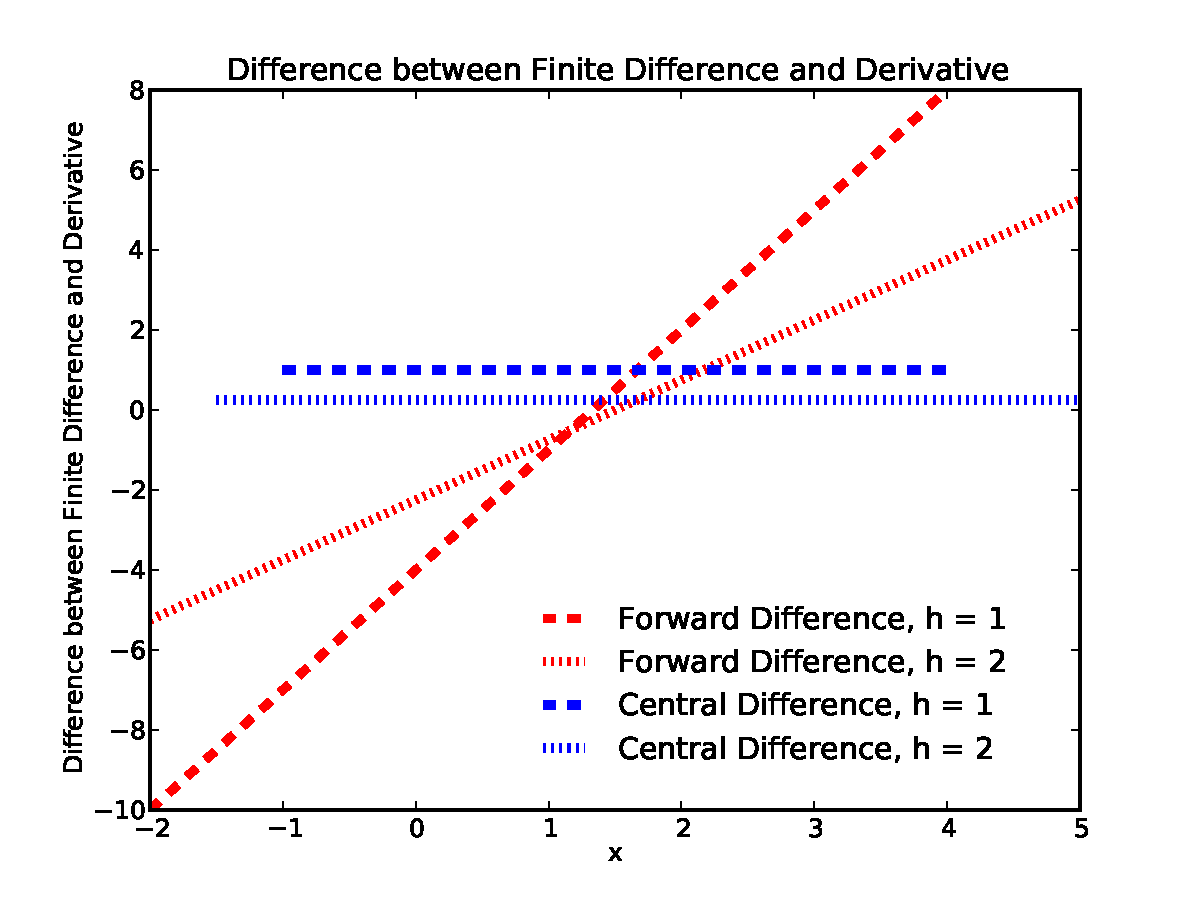
\includegraphics[width=\textwidth]{problem2_fig1.pdf}
 \caption{A plot of \(f'(x;h) - f'(x)\), or the difference between the finite difference of \(f(x) = x^3 - 5x^2 + x\) and the derivative of that function, on the interval \([-2,6]\) for both forward differencing and central differencing, each at two values of the step-size \(h\).}
\end{figure} 

\begin{figure}[H]
 \label{fig2-2}
 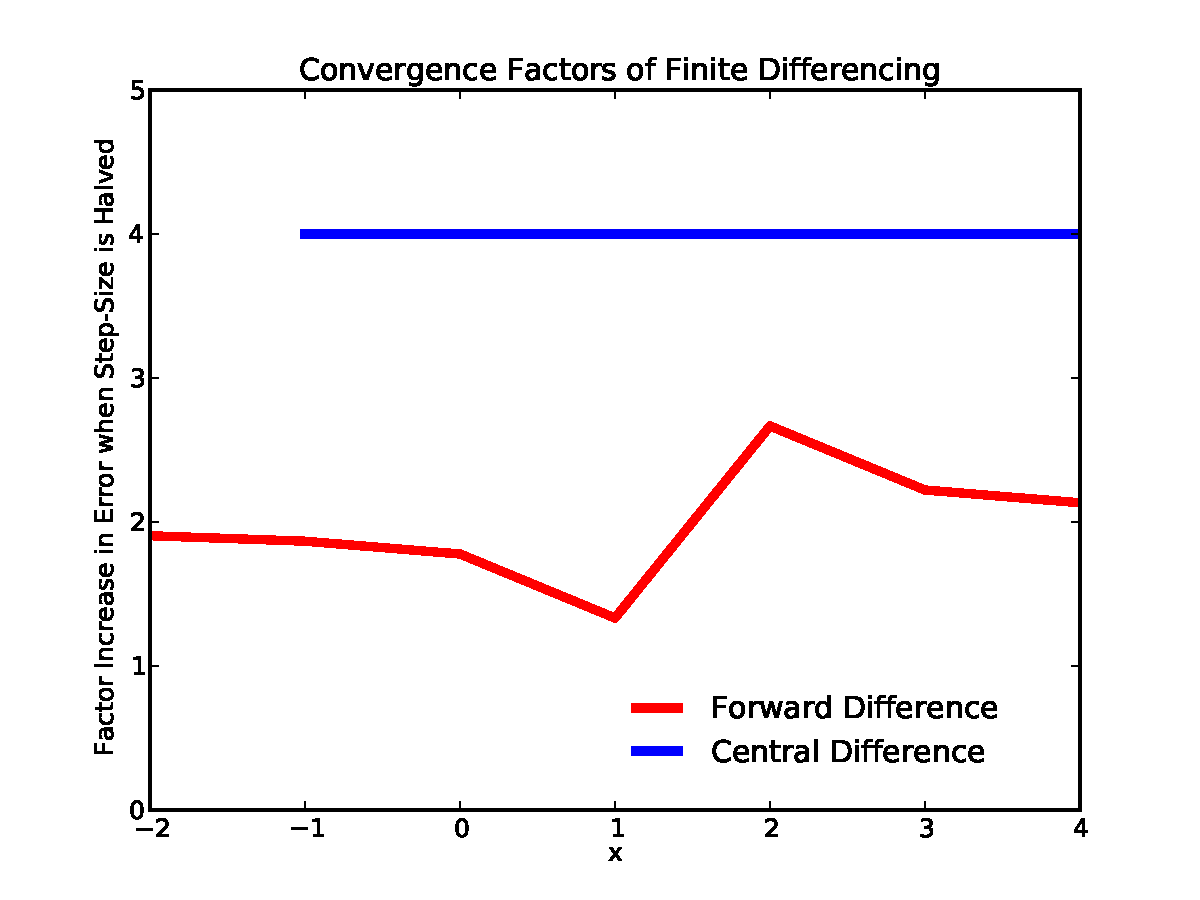
\includegraphics[width=\textwidth]{problem2_fig2.pdf}
 \caption{A plot of the ratios of the differencing errors between \(h_1 = 1\) and \(h_2 = 2\), for both forward and central differencing. We expect these ratios to be equal to the convergence factor \(\left( \frac{h_2}{h_1} \right)^n = 2^n\), where \(n\) is the convergence order of the finite differencing: \(n = 1\) for forward differencing and \(n = 2\) for central differencing. Indeed, we see that the ratio is approximately 2 for forward differencing and 4 for central differencing as expected.}
\end{figure} 

\newpage

\subsection{3. Second Derivative}

\[
f(x+h) = f(x) + h f'(x) + \frac{h^2}{2} f''(x) + \frac{h^3}{6} f'''(x) + \mathcal{O}(h^4)
\]
\[
f(x-h) = f(x) - h f'(x) + \frac{h^2}{2} f''(x) - \frac{h^3}{6} f'''(x) + \mathcal{O}(h^4)
\]
\[
\Rightarrow f(x+h) + f(x-h) = 2f(x) + h^2 f''(x) + \mathcal{O}(h^4)
\]
\begin{equation}
\boxed{f''(x) = \frac{f(x+h) - 2f(x) + f(x-h)}{h^2} + \mathcal{O}(h^2)}
\end{equation}

\vspace{1cm}

\subsection{4. Interpolation: Cepheid Lightcurve}

\begin{figure}[H]
 \label{fig4-1}
 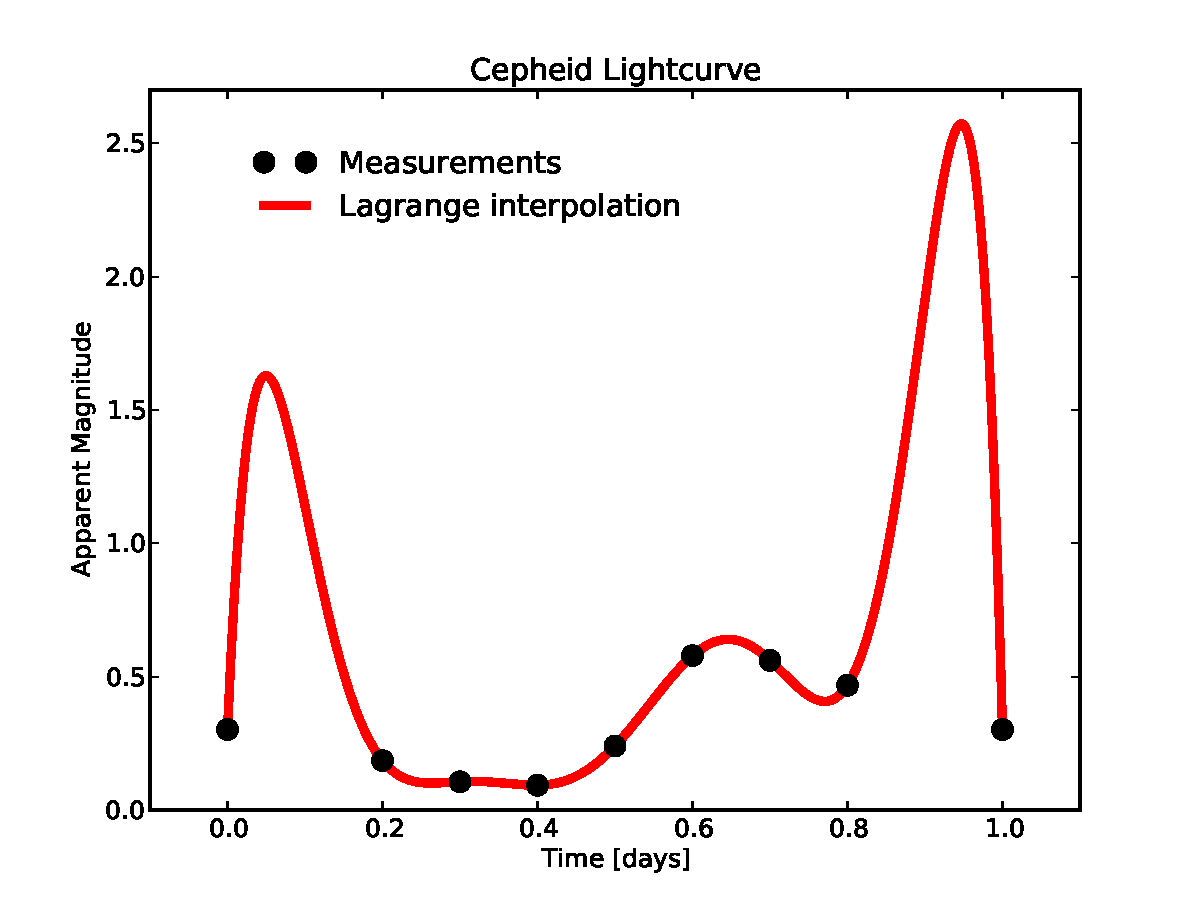
\includegraphics[width=\textwidth]{problem4_fig1.pdf}
 \caption{Apparent magnitude versus time for a Cepheid star. Actual measurements are represented as black points. Drawn in red is a Lagrange interpolation through the data.}
\end{figure} 

\begin{figure}[H]
 \label{fig4-2}
 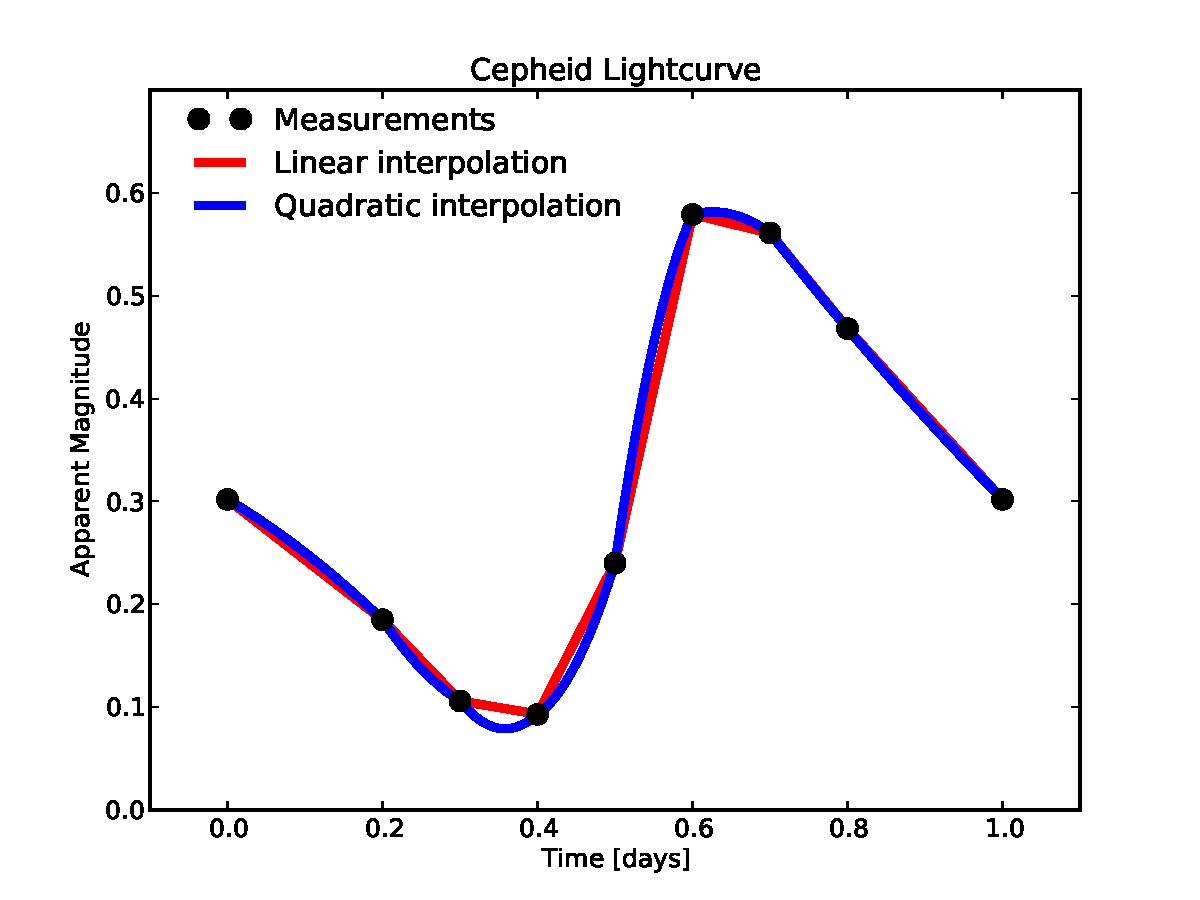
\includegraphics[width=\textwidth]{problem4_fig2.pdf}
 \caption{Apparent magnitude versus time for a Cepheid star. Actual measurements are represented as black points. Drawn in red is a piecewise-linear interpolation through the data, and drawn in blue is a piecewise-quadratic interpolation through the data.}
\end{figure} 

\subsection{5. More Cepheid Lightcurve Interpolation}

\begin{figure}[H]
 \label{fig5-1}
 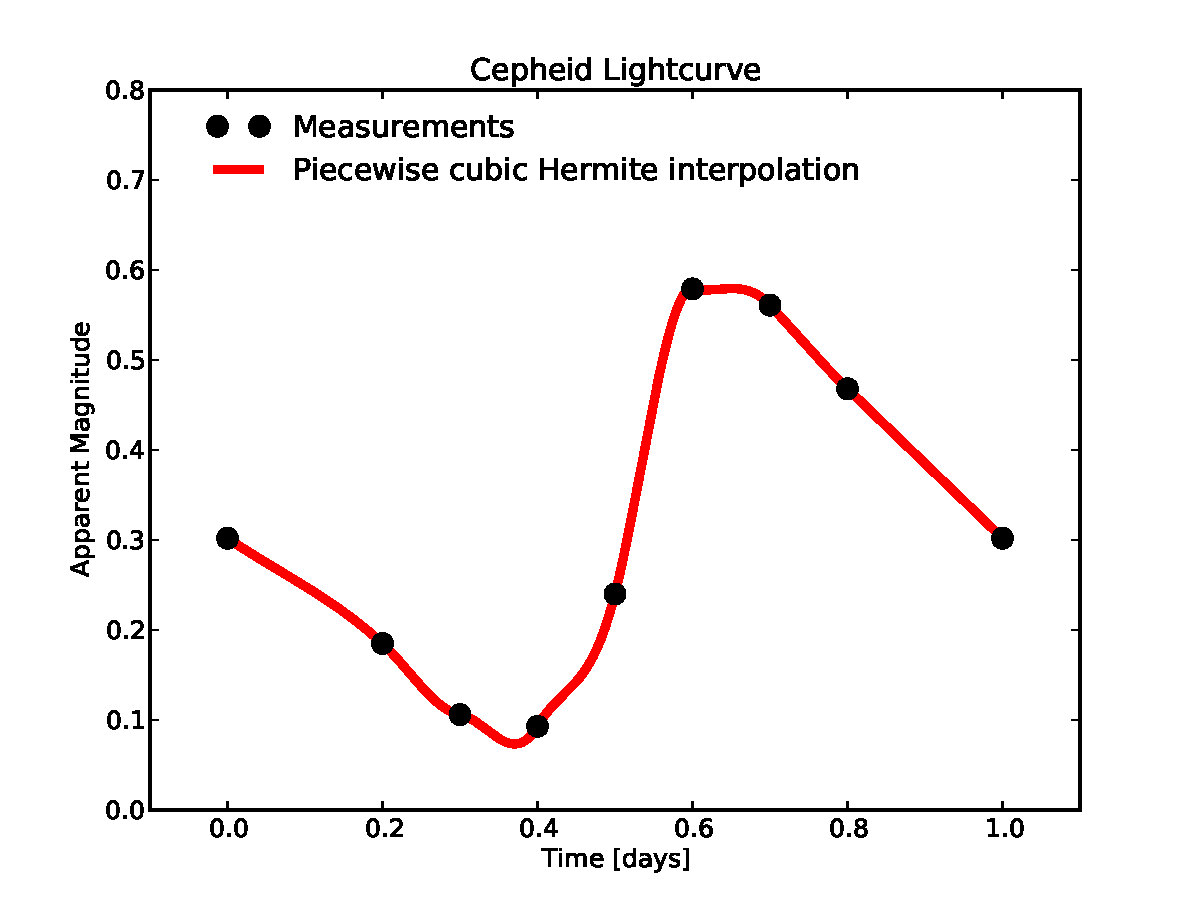
\includegraphics[width=\textwidth]{problem5_fig1.pdf}
 \caption{Apparent magnitude versus time for a Cepheid star. Actual measurements are represented as black points. Drawn in red is a piecewise cubic Hermite interpolation through the data.}
\end{figure} 

\begin{figure}[H]
 \label{fig5-2}
 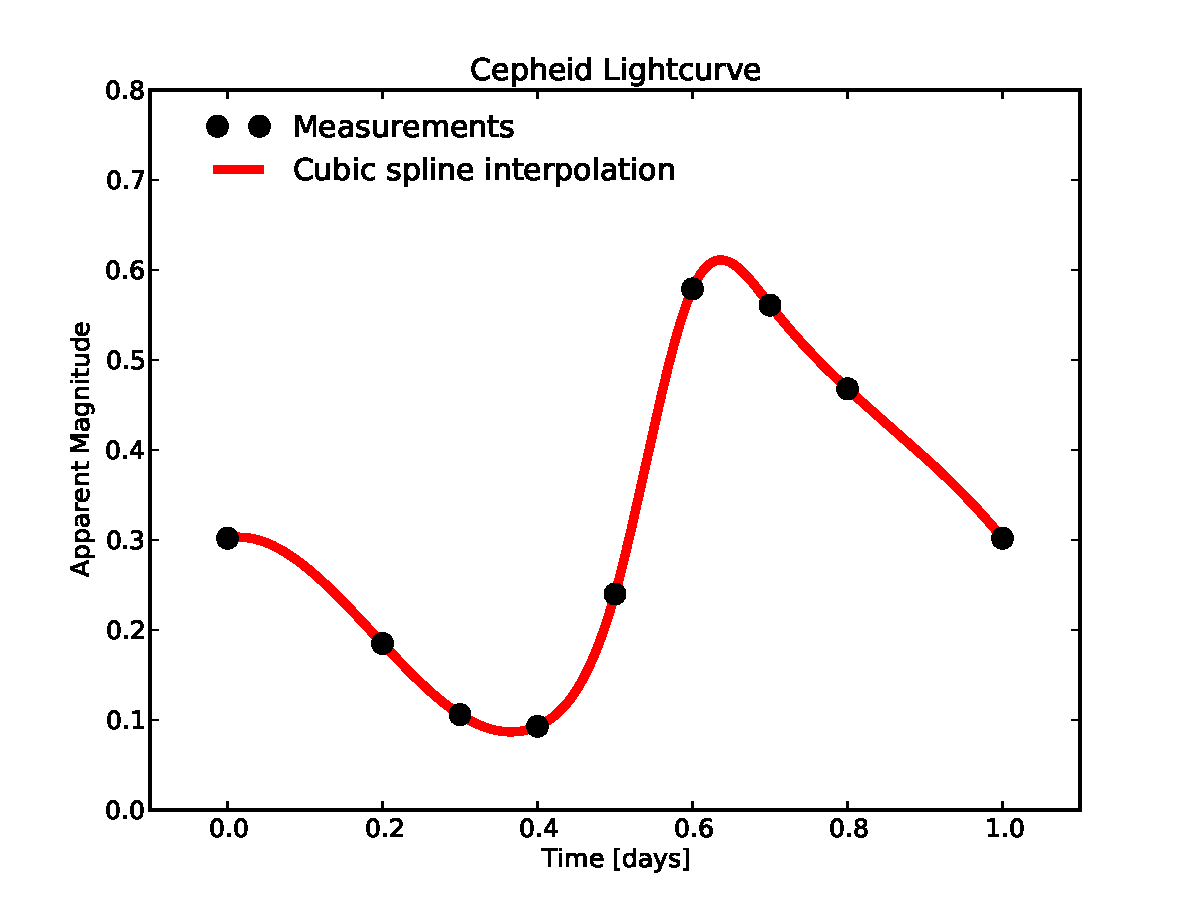
\includegraphics[width=\textwidth]{problem5_fig2.pdf}
 \caption{Apparent magnitude versus time for a Cepheid star. Actual measurements are represented as black points. Drawn in red is a cubic spline interpolation through the data.}
\end{figure} 

\subsection{Comments on the Various Interpolations}

The Lagrange interpolation looks nice in the middle of the data, but near the ends it clearly becomes pathologically oscillatory, which is unreasonable. Linear interpolation is more reasonable, but quadratic interpolation is even nicer-looking. Cubic Hermite interpolation looks a little unnatural, with jerky changes within the intervals. The nicest-looking and more reasonable interpolation here is cubic spline.

\end{spacing}
\end{document}

%%%%%%%%%%%%%%%%%%%%%%%%%%%%%%%%%%%%%%%%%%%%%%%%%%%%%%%%%%%%%
